\documentclass[11pt,addpoints,answers]{exam}
%\documentclass[11pt]{article}
\usepackage[margin=1in]{geometry}
\usepackage{amsmath, amsfonts}
\usepackage{enumerate}
\usepackage{graphicx}
\usepackage{titling}
\usepackage{url}
\usepackage{xfrac}
% \usepackage{fancyhdr} % CONFLICTS with the exam class
\usepackage{geometry}
\usepackage{graphicx}
\usepackage{natbib}
\usepackage{amsmath}
\usepackage{amssymb}
\usepackage{amsthm}
\usepackage{paralist}
\usepackage{epstopdf}
\usepackage{tabularx}
\usepackage{longtable}
\usepackage{multirow}
\usepackage{multicol}
\usepackage[colorlinks=true,urlcolor=blue]{hyperref}
\usepackage{fancyvrb}
\usepackage{algorithm}
\usepackage{algorithmic}
\usepackage{float}
\usepackage{paralist}
\usepackage[svgname]{xcolor}
\usepackage{enumerate}
\usepackage{array}
\usepackage{times}
\usepackage{url}
\usepackage{comment}
\usepackage{environ}
\usepackage{times}
\usepackage{textcomp}
\usepackage{caption}
\usepackage[colorlinks=true,urlcolor=blue]{hyperref}
\usepackage{listings}
\usepackage{parskip} % For NIPS style paragraphs.
\usepackage[compact]{titlesec} % Less whitespace around titles
\usepackage[inline]{enumitem} % For inline enumerate* and itemize*
\usepackage{datetime}
\usepackage{comment}
% \usepackage{minted}
\usepackage{lastpage}
\usepackage{color}
\usepackage{xcolor}
\usepackage{listings}
\usepackage{tikz}
\usetikzlibrary{shapes,decorations}
%\usepackage{framed}
\usepackage{booktabs}
\usepackage{cprotect}
\usepackage{xcolor}
\usepackage{verbatimbox}
\usepackage[many]{tcolorbox}
\usepackage{cancel}
\usepackage{wasysym}
\usepackage{subfigure}


%%%%%%%%%%%%%%%%%%%%%%%%%%%%%%%%%%%%%%%%%%%
% Better numbering                        %
%%%%%%%%%%%%%%%%%%%%%%%%%%%%%%%%%%%%%%%%%%%

\numberwithin{equation}{section} % Number equations within sections (i.e. 1.1, 1.2, 2.1, 2.2 instead of 1, 2, 3, 4)
\numberwithin{figure}{section} % Number figures within sections (i.e. 1.1, 1.2, 2.1, 2.2 instead of 1, 2, 3, 4)
\numberwithin{table}{section} % Number tables within sections (i.e. 1.1, 1.2, 2.1, 2.2 instead of 1, 2, 3, 4)


%%%%%%%%%%%%%%%%%%%%%%%%%%%%%%%%%%%%%%%%%%%
% Common Math Commands                    %
%%%%%%%%%%%%%%%%%%%%%%%%%%%%%%%%%%%%%%%%%%%
\newcommand{\vc}[1]{\boldsymbol{#1}}
\newcommand{\adj}[1]{\frac{d J}{d #1}}
\newcommand{\chain}[2]{\adj{#2} = \adj{#1}\frac{d #1}{d #2}}

% mathcal
\newcommand{\Ac}{\mathcal{A}}
\newcommand{\Bc}{\mathcal{B}}
\newcommand{\Cc}{\mathcal{C}}
\newcommand{\Dc}{\mathcal{D}}
\newcommand{\Ec}{\mathcal{E}}
\newcommand{\Fc}{\mathcal{F}}
\newcommand{\Gc}{\mathcal{G}}
\newcommand{\Hc}{\mathcal{H}}
\newcommand{\Ic}{\mathcal{I}}
\newcommand{\Jc}{\mathcal{J}}
\newcommand{\Kc}{\mathcal{K}}
\newcommand{\Lc}{\mathcal{L}}
\newcommand{\Mc}{\mathcal{M}}
\newcommand{\Nc}{\mathcal{N}}
\newcommand{\Oc}{\mathcal{O}}
\newcommand{\Pc}{\mathcal{P}}
\newcommand{\Qc}{\mathcal{Q}}
\newcommand{\Rc}{\mathcal{R}}
\newcommand{\Sc}{\mathcal{S}}
\newcommand{\Tc}{\mathcal{T}}
\newcommand{\Uc}{\mathcal{U}}
\newcommand{\Vc}{\mathcal{V}}
\newcommand{\Wc}{\mathcal{W}}
\newcommand{\Xc}{\mathcal{X}}
\newcommand{\Yc}{\mathcal{Y}}
\newcommand{\Zc}{\mathcal{Z}}

% mathbb
\newcommand{\Ab}{\mathbb{A}}
\newcommand{\Bb}{\mathbb{B}}
\newcommand{\Cb}{\mathbb{C}}
\newcommand{\Db}{\mathbb{D}}
\newcommand{\Eb}{\mathbb{E}}
\newcommand{\Fb}{\mathbb{F}}
\newcommand{\Gb}{\mathbb{G}}
\newcommand{\Hb}{\mathbb{H}}
\newcommand{\Ib}{\mathbb{I}}
\newcommand{\Jb}{\mathbb{J}}
\newcommand{\Kb}{\mathbb{K}}
\newcommand{\Lb}{\mathbb{L}}
\newcommand{\Mb}{\mathbb{M}}
\newcommand{\Nb}{\mathbb{N}}
\newcommand{\Ob}{\mathbb{O}}
\newcommand{\Pb}{\mathbb{P}}
\newcommand{\Qb}{\mathbb{Q}}
\newcommand{\Rb}{\mathbb{R}}
\newcommand{\Sb}{\mathbb{S}}
\newcommand{\Tb}{\mathbb{T}}
\newcommand{\Ub}{\mathbb{U}}
\newcommand{\Vb}{\mathbb{V}}
\newcommand{\Wb}{\mathbb{W}}
\newcommand{\Xb}{\mathbb{X}}
\newcommand{\Yb}{\mathbb{Y}}
\newcommand{\Zb}{\mathbb{Z}}

% mathbf lowercase
\newcommand{\av}{\mathbf{a}}
\newcommand{\bv}{\mathbf{b}}
\newcommand{\cv}{\mathbf{c}}
\newcommand{\dv}{\mathbf{d}}
\newcommand{\ev}{\mathbf{e}}
\newcommand{\fv}{\mathbf{f}}
\newcommand{\gv}{\mathbf{g}}
\newcommand{\hv}{\mathbf{h}}
\newcommand{\iv}{\mathbf{i}}
\newcommand{\jv}{\mathbf{j}}
\newcommand{\kv}{\mathbf{k}}
\newcommand{\lv}{\mathbf{l}}
\newcommand{\mv}{\mathbf{m}}
\newcommand{\nv}{\mathbf{n}}
\newcommand{\ov}{\mathbf{o}}
\newcommand{\pv}{\mathbf{p}}
\newcommand{\qv}{\mathbf{q}}
\newcommand{\rv}{\mathbf{r}}
\newcommand{\sv}{\mathbf{s}}
\newcommand{\tv}{\mathbf{t}}
\newcommand{\uv}{\mathbf{u}}
\newcommand{\vv}{\mathbf{v}}
\newcommand{\wv}{\mathbf{w}}
\newcommand{\xv}{\mathbf{x}}
\newcommand{\yv}{\mathbf{y}}
\newcommand{\zv}{\mathbf{z}}

% mathbf uppercase
\newcommand{\Av}{\mathbf{A}}
\newcommand{\Bv}{\mathbf{B}}
\newcommand{\Cv}{\mathbf{C}}
\newcommand{\Dv}{\mathbf{D}}
\newcommand{\Ev}{\mathbf{E}}
\newcommand{\Fv}{\mathbf{F}}
\newcommand{\Gv}{\mathbf{G}}
\newcommand{\Hv}{\mathbf{H}}
\newcommand{\Iv}{\mathbf{I}}
\newcommand{\Jv}{\mathbf{J}}
\newcommand{\Kv}{\mathbf{K}}
\newcommand{\Lv}{\mathbf{L}}
\newcommand{\Mv}{\mathbf{M}}
\newcommand{\Nv}{\mathbf{N}}
\newcommand{\Ov}{\mathbf{O}}
\newcommand{\Pv}{\mathbf{P}}
\newcommand{\Qv}{\mathbf{Q}}
\newcommand{\Rv}{\mathbf{R}}
\newcommand{\Sv}{\mathbf{S}}
\newcommand{\Tv}{\mathbf{T}}
\newcommand{\Uv}{\mathbf{U}}
\newcommand{\Vv}{\mathbf{V}}
\newcommand{\Wv}{\mathbf{W}}
\newcommand{\Xv}{\mathbf{X}}
\newcommand{\Yv}{\mathbf{Y}}
\newcommand{\Zv}{\mathbf{Z}}

% bold greek lowercase
\newcommand{\alphav     }{\boldsymbol \alpha     }
\newcommand{\betav      }{\boldsymbol \beta      }
\newcommand{\gammav     }{\boldsymbol \gamma     }
\newcommand{\deltav     }{\boldsymbol \delta     }
\newcommand{\epsilonv   }{\boldsymbol \epsilon   }
\newcommand{\varepsilonv}{\boldsymbol \varepsilon}
\newcommand{\zetav      }{\boldsymbol \zeta      }
\newcommand{\etav       }{\boldsymbol \eta       }
\newcommand{\thetav     }{\boldsymbol \theta     }
\newcommand{\varthetav  }{\boldsymbol \vartheta  }
\newcommand{\iotav      }{\boldsymbol \iota      }
\newcommand{\kappav     }{\boldsymbol \kappa     }
\newcommand{\varkappav  }{\boldsymbol \varkappa  }
\newcommand{\lambdav    }{\boldsymbol \lambda    }
\newcommand{\muv        }{\boldsymbol \mu        }
\newcommand{\nuv        }{\boldsymbol \nu        }
\newcommand{\xiv        }{\boldsymbol \xi        }
\newcommand{\omicronv   }{\boldsymbol \omicron   }
\newcommand{\piv        }{\boldsymbol \pi        }
\newcommand{\varpiv     }{\boldsymbol \varpi     }
\newcommand{\rhov       }{\boldsymbol \rho       }
\newcommand{\varrhov    }{\boldsymbol \varrho    }
\newcommand{\sigmav     }{\boldsymbol \sigma     }
\newcommand{\varsigmav  }{\boldsymbol \varsigma  }
\newcommand{\tauv       }{\boldsymbol \tau       }
\newcommand{\upsilonv   }{\boldsymbol \upsilon   }
\newcommand{\phiv       }{\boldsymbol \phi       }
\newcommand{\varphiv    }{\boldsymbol \varphi    }
\newcommand{\chiv       }{\boldsymbol \chi       }
\newcommand{\psiv       }{\boldsymbol \psi       }
\newcommand{\omegav     }{\boldsymbol \omega     }

% bold greek uppercase
\newcommand{\Gammav     }{\boldsymbol \Gamma     }
\newcommand{\Deltav     }{\boldsymbol \Delta     }
\newcommand{\Thetav     }{\boldsymbol \Theta     }
\newcommand{\Lambdav    }{\boldsymbol \Lambda    }
\newcommand{\Xiv        }{\boldsymbol \Xi        }
\newcommand{\Piv        }{\boldsymbol \Pi        }
\newcommand{\Sigmav     }{\boldsymbol \Sigma     }
\newcommand{\Upsilonv   }{\boldsymbol \Upsilon   }
\newcommand{\Phiv       }{\boldsymbol \Phi       }
\newcommand{\Psiv       }{\boldsymbol \Psi       }
\newcommand{\Omegav     }{\boldsymbol \Omega     }

%%%%%%%%%%%%%%%%%%%%%%%%%%%%%%%%%%%%%%%%%%%
% Code highlighting with listings         %
%%%%%%%%%%%%%%%%%%%%%%%%%%%%%%%%%%%%%%%%%%%

\definecolor{bluekeywords}{rgb}{0.13,0.13,1}
\definecolor{greencomments}{rgb}{0,0.5,0}
\definecolor{redstrings}{rgb}{0.9,0,0}
\definecolor{light-gray}{gray}{0.95}

\newcommand{\MYhref}[3][blue]{\href{#2}{\color{#1}{#3}}}%

\definecolor{dkgreen}{rgb}{0,0.6,0}
\definecolor{gray}{rgb}{0.5,0.5,0.5}
\definecolor{mauve}{rgb}{0.58,0,0.82}

\lstdefinelanguage{Shell}{
  keywords={tar, cd, make},
  %keywordstyle=\color{bluekeywords}\bfseries,
  alsoletter={+},
  ndkeywords={python, py, javac, java, gcc, c, g++, cpp, .txt, octave, m, .tar},
  %ndkeywordstyle=\color{bluekeywords}\bfseries,
  identifierstyle=\color{black},
  sensitive=false,
  comment=[l]{//},
  morecomment=[s]{/*}{*/},
  commentstyle=\color{purple}\ttfamily,
  stringstyle=\color{red}\ttfamily,
  morestring=[b]',
  morestring=[b]",
  backgroundcolor = \color{light-gray}
}

\lstset{columns=fixed, basicstyle=\ttfamily,
    backgroundcolor=\color{light-gray},xleftmargin=0.5cm,frame=tlbr,framesep=4pt,framerule=0pt}


%%%%%%%%%%%%%%%%%%%%%%%%%%%%%%%%%%%%%%%%%%%
% Custom box for highlights               %
%%%%%%%%%%%%%%%%%%%%%%%%%%%%%%%%%%%%%%%%%%%

% Define box and box title style
\tikzstyle{mybox} = [fill=blue!10, very thick,
    rectangle, rounded corners, inner sep=1em, inner ysep=1em]

% \newcommand{\notebox}[1]{
% \begin{tikzpicture}
% \node [mybox] (box){%
%     \begin{minipage}{\textwidth}
%     #1
%     \end{minipage}
% };
% \end{tikzpicture}%
% }

\NewEnviron{notebox}{
\begin{tikzpicture}
\node [mybox] (box){
    \begin{minipage}{\textwidth}
        \BODY
    \end{minipage}
};
\end{tikzpicture}
}

%%%%%%%%%%%%%%%%%%%%%%%%%%%%%%%%%%%%%%%%%%%
% Commands showing / hiding solutions     %
%%%%%%%%%%%%%%%%%%%%%%%%%%%%%%%%%%%%%%%%%%%

%% To HIDE SOLUTIONS (to post at the website for students), set this value to 0: \def\issoln{0}
\def\issoln{0}
% Some commands to allow solutions to be embedded in the assignment file.
\ifcsname issoln\endcsname \else \def\issoln{0} \fi
% Default to an empty solutions environ.
\NewEnviron{soln}{}{}
% Default to an empty qauthor environ.
\NewEnviron{qauthor}{}{}
% Default to visible (but empty) solution box.
\newtcolorbox[]{studentsolution}[1][]{%
    breakable,
    enhanced,
    colback=white,
    title=Solution,
    #1
}

\if\issoln 1
% Otherwise, include solutions as below.
\RenewEnviron{soln}{
    \leavevmode\color{red}\ignorespaces
    \textbf{Solution} \BODY
}{}
\fi

\if\issoln 1
% Otherwise, include solutions as below.
\RenewEnviron{solution}{}
\fi

%%%%%%%%%%%%%%%%%%%%%%%%%%%%%%%%%%%%%%%%%%%
% Commands for customizing the assignment %
%%%%%%%%%%%%%%%%%%%%%%%%%%%%%%%%%%%%%%%%%%%

\newcommand{\courseNum}{10-418 / 10-618}
\newcommand{\courseName}{Machine Learning for Structured Data}
\newcommand{\courseSem}{Fall 2019}
\newcommand{\piazzaUrl}{\url{https://piazza.com/cmu/fall2019/1041810618}}
\newcommand{\hwNum}{Homework 1}
\newcommand{\hwTopic}{Learning to Search}
\newcommand{\hwName}{\hwNum: \hwTopic}
\newcommand{\outDate}{Sep. 13, 2019}
\newcommand{\dueDate}{Sep. 26, 2019 11:59 PM}
\newcommand{\taNames}{Austin, Karthika, Aakanksha}

%\pagestyle{fancyplain}
\lhead{\hwName}
\rhead{\courseNum}
\cfoot{\thepage{} of \numpages{}}

\title{\textsc{\hwName}} % Title

\date{}

%%%%%%%%%%%%%%%%%%%%%%%%%%%%%%%%%%%%%%%%%%%%%%%%%
% Useful commands for typesetting the questions %
%%%%%%%%%%%%%%%%%%%%%%%%%%%%%%%%%%%%%%%%%%%%%%%%%

\newcommand \expect {\mathbb{E}}
\newcommand \mle [1]{{\hat #1}^{\rm MLE}}
\newcommand \map [1]{{\hat #1}^{\rm MAP}}
\newcommand \argmax {\operatorname*{argmax}}
\newcommand \argmin {\operatorname*{argmin}}
\newcommand \code [1]{{\tt #1}}
\newcommand \datacount [1]{\#\{#1\}}
\newcommand \ind [1]{\mathbb{I}\{#1\}}

\newcommand{\blackcircle}{\tikz\draw[black,fill=black] (0,0) circle (1ex);}
\renewcommand{\circle}{\tikz\draw[black] (0,0) circle (1ex);}

\newcommand{\pts}[1]{\textbf{[#1 pts]}}

%%%%%%%%%%%%%%%%%%%%%%%%%%
% Document configuration %
%%%%%%%%%%%%%%%%%%%%%%%%%%

% Don't display a date in the title and remove the white space
\predate{}
\postdate{}
\date{}

% Don't display an author and remove the white space
%\preauthor{}
%\postauthor{}

%%%%%%%%%%%%%%%%%%
% Begin Document %
%%%%%%%%%%%%%%%%%% 


\begin{document}

\section*{}
\begin{center}
  \textsc{\LARGE \hwNum} \\
  \textsc{\LARGE \hwTopic\footnote{Compiled on \today{} at \currenttime{}}} \\
  \vspace{1em}
  \textsc{\large \courseNum{} \courseName{} (\courseSem)} \\
  %\vspace{0.25em}
  \piazzaUrl\\
  \vspace{1em}
  OUT: \outDate \\
  %\vspace{0.5em}
  DUE: \dueDate \\
  TAs: \taNames
\end{center}


\section*{START HERE: Instructions}

\begin{notebox}
\paragraph{Summary} In this assignment, you will implement a Seq2Seq trained with the Maximum Likelihood Estimation and DAgger for automatically transcibing audio recordings to text. As a warmup, Section \ref{sec:warmup} will lead you through an on-paper example of learning to search and recurrent neural network language models. Then, in Section \ref{sec:code}, you will implement a simple Seq2Seq model and analyze its performance.
\end{notebox}

\begin{itemize}
\item \textbf{Collaboration policy:} Collaboration on solving the homework is allowed, after you have thought about the problems on your own. It is also OK to get clarification (but not solutions) from books or online resources, again after you have thought about the problems on your own. There are two requirements: first, cite your collaborators fully and completely (e.g., ``Jane explained to me what is asked in Question 2.1''). Second, write your solution {\em independently}: close the book and all of your notes, and send collaborators out of the room, so that the solution comes from you only.  See the Academic Integrity Section on the course site for more information: \url{http://www.cs.cmu.edu/~mgormley/courses/10418/about.html#7-academic-integrity-policies}

\item\textbf{Late Submission Policy:} See the late submission policy here: \url{http://www.cs.cmu.edu/~mgormley/courses/10418/about.html#6-general-policies}

\item \textbf{Autolab:} You will submit your code for programming questions on the homework to Autolab (\url{https://autolab.andrew.cmu.edu/}). After uploading your code,
we will manually grade your code by hand. We will not use Autolab to autograde your code.

\item \textbf{Submitting your work to Gradescope:} For written problems such as short answer, multiple choice, derivations, proofs, or plots, we will be using Gradescope (\url{https://gradescope.com/}). Please use the provided template. Submissions can be handwritten, but should be labeled and clearly legible. If your writing is not legible, you will not be awarded marks. Alternatively, submissions can be written in LaTeX. Regrade requests can be made, however this gives the TA the opportunity to regrade your entire paper, meaning if additional mistakes are found then points will be deducted. For short answer questions you \textbf{should not} include your work in your solution.  If you include your work in your solutions, your assignment may not be graded correctly by our AI assisted grader. 

\end{itemize}

For multiple choice or select all that apply questions, shade in the box or circle in the template document corresponding to the correct answer(s) for each of the questions. For \LaTeX users, use $\blacksquare$ and \blackcircle  for shaded boxes and circles, and don't change anything else.



\clearpage

%Written Portion
\section{Written Questions}
\label{sec:warmup}
Answer the following questions in the template provided.  Then upload your solutions to Gradescope. You may use \LaTeX\ or print the template and hand-write your answers then scan it in. Failure to use the template may result in a penalty.

\subsection{Reductions to Binary Classification}

\begin{questions}
\question[1] Can we construct an ECOC matrix that yields the same algorithm as One vs. All classification? \emph{If yes, describe the matrix; if not, explain why not.}
\begin{tcolorbox}[fit,height=2cm, width=15cm, blank, borderline={1pt}{-2pt}]
    % STUDENT SOLUTION HERE
    \end{tcolorbox}
    
\question[1] Can we construct an ECOC matrix that yields the same algorithm as All vs. All classification? \emph{If yes, describe the matrix; if not, explain why not.}
\begin{tcolorbox}[fit,height=2cm, width=15cm, blank, borderline={1pt}{-2pt}]
    % STUDENT SOLUTION HERE
    \end{tcolorbox}


\question[1] \textbf{True or False:} One-against-some classifier has logarithmic runtime in the number of examples.
    \begin{checkboxes}
     \choice True 
     \choice False
    \end{checkboxes}
    
\question[1] \textbf{True or False:} Extreme classification assumes a large label set.
    \begin{checkboxes}
     \choice True 
     \choice False
    \end{checkboxes}
 
\question[2] For a full binary classification tree of depth $d$, what is the probability of making a correct classification on  $\vec{X}$. Assume that the probability of a binary classifier at any node making an error is $\epsilon$. (A full binary tree is one in which every node, except the leaves, has two children.)
\begin{tcolorbox}[fit,height=2cm, width=15cm, blank, borderline={1pt}{-2pt}]
    % STUDENT SOLUTION HERE
    \end{tcolorbox}
\question \textbf{Numerical answer:} For $k$-way multi-classification with $k=16$, how many classifiers need to be constructed for...
\begin{parts}
\part[1] ...One vs. All classification?
    \begin{tcolorbox}[fit,height=1cm, width=2cm, blank, borderline={1pt}{-2pt}]
    % STUDENT SOLUTION HERE
    \end{tcolorbox}
\part[1] ...All vs. All classification?
    \begin{tcolorbox}[fit,height=1cm, width=2cm, blank, borderline={1pt}{-2pt}]
    % STUDENT SOLUTION HERE
    \end{tcolorbox}
\end{parts}

\question[1] For an arbitrary classification tree with $k$ classes, what is the minimum number of binary classifiers that could be needed?
    \begin{tcolorbox}[fit,height=1cm, width=2cm, blank, borderline={1pt}{-2pt}]
    % STUDENT SOLUTION HERE
    \end{tcolorbox}
    
\question[1] For an arbitrary classification tree with $k$ classes, What is the maximum number of classifiers that could be needed? (Assume that the sets of classes for each pair of siblings are mutually exclusive.)
    \begin{tcolorbox}[fit,height=1cm, width=2cm, blank, borderline={1pt}{-2pt}]
    % STUDENT SOLUTION HERE
    \end{tcolorbox}


\end{questions}

\clearpage
\subsection{Learning to Search}

In this section, we'll consider a simple version of learning to search for the task of identifying names in a text. In this setting our action space will be the set $\{ +, -\}$ where $+$ denotes labeling a word as part of a name and $-$ denotes labeling a word as not being part of a name. Our state space will be represented by $S_z$ where $z$ is a vector denoting the labeling of our sentence so far. For example, if we are in state $S_{++-}$ it means we have labeled word 0 as $+$, word 1 as $+$, word 2 as $-$, and we are currently attempting to label word 3. 

Throughout this section, we will be referring exclusively to the following input sentence $\vec{x}$ and oracle labeling $\vec{y}$:

\begin{figure}[h]
\centering

\includegraphics[width=0.75\linewidth]{fig/x.jpg}
\label{example_sentence}
\end{figure}

In Figure \ref{state_space} you can see a small part of the search space for this problem. 

\begin{figure}[h]
\centering
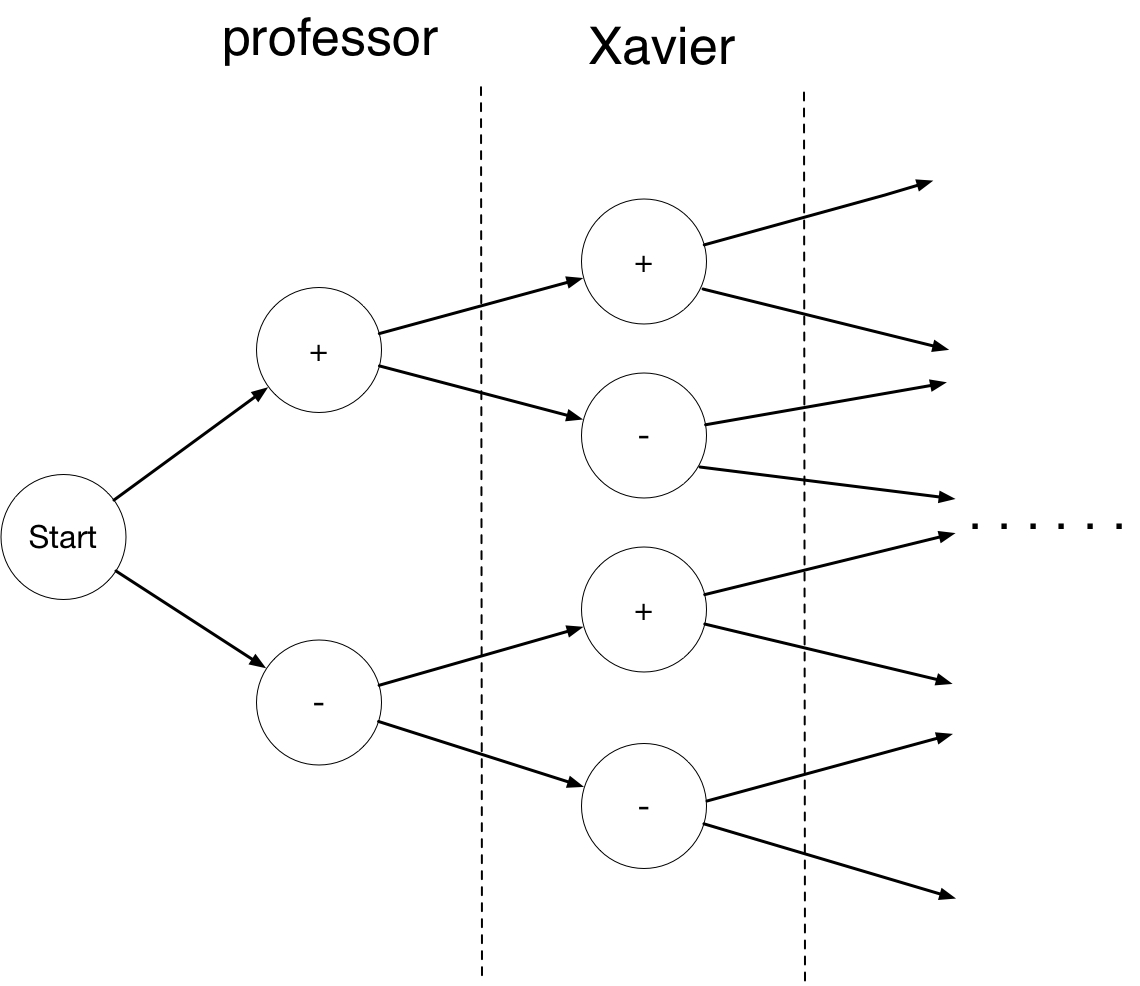
\includegraphics[width=0.5\linewidth]{fig/state_space.jpg}
\caption{}
\label{state_space}
\end{figure}

\begin{questions}
\question[1] How many nodes are in the search space for sentence $\vec{x}$?
    \begin{tcolorbox}[fit,height=1cm, width=2cm, blank, borderline={1pt}{-2pt}]
    % STUDENT SOLUTION HERE
    \end{tcolorbox}

\question[1] How many nodes are in the search space for a sentence of length $T$?
    \begin{tcolorbox}[fit,height=2cm, width=15cm, blank, borderline={1pt}{-2pt}]
    % STUDENT SOLUTION HERE
    \end{tcolorbox}

\clearpage
\question Suppose our loss function is Hamming loss.

\begin{parts}
\part[1] What does the oracle policy return for $S_{++-}$?
    \begin{tcolorbox}[fit,height=2cm, width=15cm, blank, borderline={1pt}{-2pt}]
    % STUDENT SOLUTION HERE
    \end{tcolorbox}
    
\part[1] What does the oracle policy return for $S_{---}$?
    \begin{tcolorbox}[fit,height=2cm, width=15cm, blank, borderline={1pt}{-2pt}]
    % STUDENT SOLUTION HERE
    \end{tcolorbox}

\end{parts}

\question Suppose our loss function is Hamming loss with an additional error for including only part of a name, e.g. omitting a person's title. More precisely, 

\begin{equation*}
    c(y, \hat{y}) =  \left [ \ \sum_{t=0}^{T-1} \ind{ y_t \neq \hat{y}_t}\right] + \left [ \ \sum_{t=1}^{T-1} \ind{ y_{t-1} = + , \hat{y}_{t-1} = -, y_t = +, \hat{y}_t = +}\right]
\end{equation*}

\begin{parts}
\part[1] What does the oracle policy return for $S_{-}$?
    \begin{tcolorbox}[fit,height=2cm, width=15cm, blank, borderline={1pt}{-2pt}]
    % STUDENT SOLUTION HERE
    \end{tcolorbox}

\part[1] What does the oracle policy return for $S_{+}$?
    \begin{tcolorbox}[fit,height=2cm, width=15cm, blank, borderline={1pt}{-2pt}]
    % STUDENT SOLUTION HERE
    \end{tcolorbox}
\end{parts}

\question Suppose that our scoring function is of the form $\thetav^T \fv(x_i, y_i)$ where 

\begin{equation*}
\begin{split}
\fv(x_i, y_i) = & [\ind{x_i \text{ starts with a capital letter and } y_i =  +} \\
& \ind{x_i \text{ starts with a capital letter and } y_i =  -}, \\
& \ind{\text{ is in our gazetteer list and } y_i = +}, \\
& \ind{\text{ is in our gazetteer list and } y_i = -}, \\
& \ind{y_{i-1} = -, y_i = -}]
\end{split}
\end{equation*}

and $\thetav$ is a vector of length 5. A gazetteer list is essentially a lookup table of entities that we know are names. Our gazetteer list will include $\{$ Xavier, Mellon $\}$. 

Assume our initial weight vector $\thetav = [-1, 1, -1, 1, 0]$. 

\begin{parts}
\part[1] What score would our scoring function assign to the ground truth labeling?
\begin{tcolorbox}[fit,height=1cm, width=2cm, blank, borderline={1pt}{-2pt}]
    % STUDENT SOLUTION HERE
    \end{tcolorbox}
    
\part[1] What labeling would the greedy policy induced by this scoring function return? Break any ties with $+$. 
\begin{tcolorbox}[fit,height=2cm, width=15cm, blank, borderline={1pt}{-2pt}]
    % STUDENT SOLUTION HERE
    \end{tcolorbox}

\part[1] Suppose we use the Supervised Approach to Imitation Learning. Which (state, action) pairs would be produced by the learning algorithm? Denote the action by either $+$ or $-$. Denote a state by the partial sequence it corresponds to (e.g. the state $+-$ corresponds to a state that took action $+$ followed by action $-$). 
\begin{tcolorbox}[fit,height=2cm, width=15cm, blank, borderline={1pt}{-2pt}]
    % STUDENT SOLUTION HERE
    \end{tcolorbox}
    

\part[1] Suppose we use DAgger, Which (state, action) pairs would be produced by the learning algorithm? Use the same denotation of states and actions as in the previous question.
\begin{tcolorbox}[fit,height=2cm, width=15cm, blank, borderline={1pt}{-2pt}]
    % STUDENT SOLUTION HERE
    \end{tcolorbox}
    
\clearpage
\begin{EnvFullwidth}
We decide to train our linear model using the Perceptron update rule. That is, if the classifier (aka. greedy policy) makes a positive mistake (i.e. a mistake where $y_i=+$) in its action selection, then we \emph{add} the feature vector to the weights. If it makes a negative mistake (i.e. a mistake where $y_i=-$), then we \emph{subtract} the feature vector from the weights. We treat the arrival of each (state, action) pair as a separate online example for the classifier.
\end{EnvFullwidth}

\part[1] Using the (state, action) pairs produced by the Supervised Approach to Imitation Learning, what would the new value of $\thetav$ be after completing the corresponding Perceptron updates?
\begin{tcolorbox}[fit,height=2cm, width=15cm, blank, borderline={1pt}{-2pt}]
    % STUDENT SOLUTION HERE
    \end{tcolorbox}

\part[1] Using the (state, action) pairs produced by DAgger, what would the new value of $\thetav$ be after completing the corresponding Perceptron updates?
\begin{tcolorbox}[fit,height=2cm, width=15cm, blank, borderline={1pt}{-2pt}]
    % STUDENT SOLUTION HERE
    \end{tcolorbox}

% TODO: Add a conceptual question about using a classifier other than Perceptorn (e.g. SVM).  

\end{parts}
\end{questions}

\clearpage
\subsection{Recurrent Neural Network Language Models}

%\begin{EnvFullwidth}

In this section, we wish to use an Elman Network as a building block to design an RNN language model. Below we define the Elman network recursively.
%
\begin{align*}
& \bv_t = \text{relu}( \Bv^T \bv_{t-1} + \Av^T \av_t + \dv ) \\
& \cv_t = \text{softmax}( \Cv^T \bv_t + \ev)
\end{align*}
%
where $\av_t, \forall t$ is given as input to the network; $\Av, \Bv, \Cv, \dv, \ev$ are parameters of the network; and the initial hidden units $\bv_0$ are also treated as parameters. In this problem, we assume $\av_t, \bv_t, \cv_t \in \Rb^2$ for all $t$, i.e. all vectors have length two, and that the parameters matrices and vectors are appropriately defined to preserve those dimensions. Above, the function $\text{relu}(\cdot)$ is the Rectified Linear Unit function applied elementwise to its vector-valued parameter. The function $\text{softmax}(\cdot)$ is likewise vector-valued and defined below. We use $[\cdot]_i$ to explicitly denote the $i$th element of its argument.
%
\begin{align*}
& [\text{relu}(\vv)]_i \triangleq \max(0, v_i) \\
& [\text{softmax}(\vv)]_i \triangleq \frac{ \exp(v_i) }{ \sum_{j=1}^M \exp(v_j) }
\end{align*}
%
Figure \ref{fig:rnnlm} depicts the Elman Network. The parameters are shown in red, but their connections into the computation graph are not shown.

\begin{figure}[H]
    \centering
    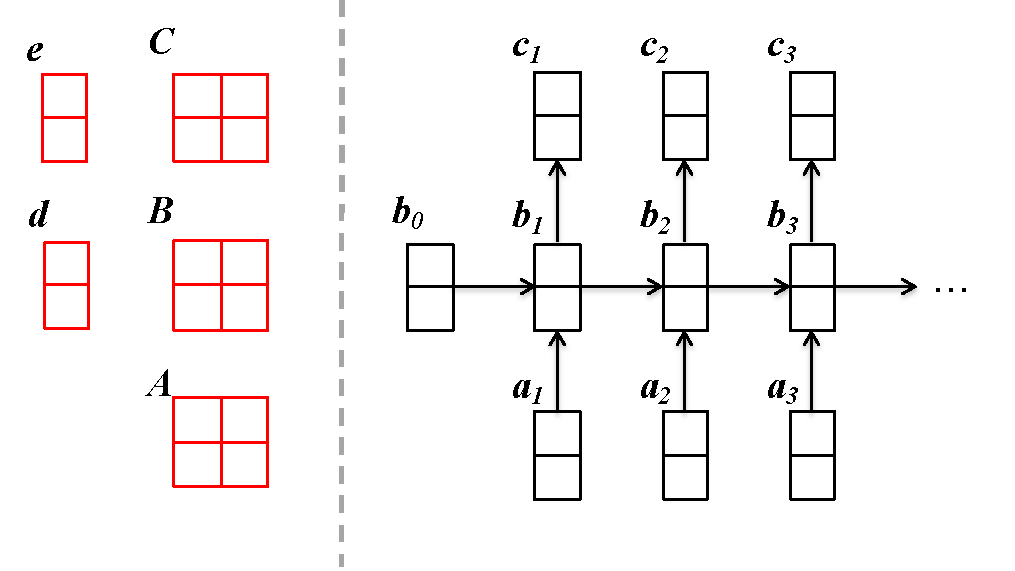
\includegraphics[width=0.8\textwidth]{fig/hw1_rnn.pdf}
    \caption{}
    \label{fig:rnnlm}
\end{figure}
%
Assume that we wish to build a language model $p(\yv)$ of binary sequences $\yv \in \{ +, - \}^L$ of fixed length $L$. We have training data consisting of sequences $\Dc = \{ \yv^{(1)}, \ldots, \yv^{(N)} \}$, , where $|\yv^{(i)}| = L$. Assume further that we have pre-encoded the data as sequences of one-hot vectors $\Dc' = \{ \zv^{(1)}, \ldots, \zv^{(N)} \}$ such that:
\begin{align*}
    & \text{ if $y^{(i)}_t = +$, then $\zv^{(i)}_t = [1, 0]^T$, } \\
    & \text{ if $y^{(i)}_t = -$, then $\zv^{(i)}_t = [0, 1]^T$. }
\end{align*}
For such a pair of vectors, we write that $\zv^{(i)} = \text{one-hot}(\yv^{(i)})$
%
%\end{EnvFullwidth}

\begin{questions}


\question[1] \textbf{Short answer:}  Since we wish to treat this Elman Network as an RNN-LM, how many inputs $\av_t$ will we need for a single training example $\yv \in \Dc$ with $|\yv| = L$? \textbf{Explain your answer.}
    \begin{tcolorbox}[fit,height=2cm, width=15cm, blank, borderline={1pt}{-2pt}]
    % STUDENT SOLUTION HERE
    \end{tcolorbox}

\question[1] \textbf{Select one:} If we decide to train this RNN-LM with \emph{Teacher Forcing}, we will need to compute a loss function for an input example $\yv \in \Dc$. Assuming so, how would we define $\av_t$? \textit{Note: Be sure to account for all $t$ in your definition.}
    \begin{tcolorbox}[fit,height=2cm, width=15cm, blank, borderline={1pt}{-2pt}]
    % STUDENT SOLUTION HERE
    \end{tcolorbox}
    
\question[1] \textbf{Select one:} If we decide to train this RNN-LM with \emph{Scheduled Sampling}, we will need to compute a loss function for an input example $\yv \in \Dc$. Assuming we use a schedule that always selects the model policy with probability 1, how would we define $\av_t$? \textit{Note: Be sure to account for all $t$ in your definition.} 
    \begin{tcolorbox}[fit,height=2cm, width=15cm, blank, borderline={1pt}{-2pt}]
    % STUDENT SOLUTION HERE
    \end{tcolorbox}
    
% TODO: Write a question about how Scheduled Sampling might be an odd choice here?
    
\question[1] Write the cross entropy loss $\ell$ for a single training example $\zv \in \Dc'$ in terms of the units and/or parameters of the RNN-LM: $\av_t, \bv_t, \cv_t, \Av, \Bv, \Cv, \dv, \ev$.
    \begin{tcolorbox}[fit,height=2cm, width=15cm, blank, borderline={1pt}{-2pt}]
    % STUDENT SOLUTION HERE
    \end{tcolorbox}
    
\begin{EnvFullwidth}
Suppose we have parameter values as defined below:
\begin{align}
& \Av = \begin{bmatrix} 1 & 1 \\ 1 & 1 \end{bmatrix} 
&& \Bv = \begin{bmatrix} 0.5 & 0.5 \\ 0.5 & 0.5 \end{bmatrix} 
&& \Cv = \begin{bmatrix} 1 & 1 \\ 2 & 1 \end{bmatrix} \\
& \dv = \begin{bmatrix} 0 \\ 0 \end{bmatrix} 
&& \ev = \begin{bmatrix} 0 \\ 0 \end{bmatrix} 
&& \bv_0 = \begin{bmatrix} 0 \\ 0 \end{bmatrix} 
\end{align}

\end{EnvFullwidth}
    

\question \textbf{Numerical answer:} When computing the probability of the sequence $\yv = [+, -, +]$, what is the value of the following three quantities? \emph{Note: Round each numerical value to two significant figures.}
\begin{parts}
    \part[1] $b_{1,1} = \quad$ 
    \begin{tcolorbox}[fit,height=1cm, width=2cm, blank, borderline={1pt}{-2pt},nobeforeafter]
    % STUDENT SOLUTION HERE
    \end{tcolorbox}
    \part[1] $b_{2,1} = \quad$ 
    \begin{tcolorbox}[fit,height=1cm, width=2cm, blank, borderline={1pt}{-2pt},nobeforeafter]
    % STUDENT SOLUTION HERE
    \end{tcolorbox}
\end{parts}
    
\question \textbf{Numerical answer:} When computing the probability of the sequence $\yv = [+, -, +]$, what is the value of the following three quantities? \emph{Note: Round each numerical value to two significant figures.}
\begin{parts}
    \part[1] $c_{1,1} = \quad$ 
    \begin{tcolorbox}[fit,height=1cm, width=2cm, blank, borderline={1pt}{-2pt},nobeforeafter]
    % STUDENT SOLUTION HERE
    \end{tcolorbox}
    \part[1] $c_{2,1} = \quad$ 
    \begin{tcolorbox}[fit,height=1cm, width=2cm, blank, borderline={1pt}{-2pt},nobeforeafter]
    % STUDENT SOLUTION HERE
    \end{tcolorbox}
\end{parts}

\question[1] \textbf{Numerical answer:} What is the probability of the sequence $\yv = [+, -, +]$ according to this RNNLM? \emph{Note: Round the numerical value to two significant figures.}
    
    $p(\yv) = \quad$
    \begin{tcolorbox}[fit,height=1cm, width=2cm, blank, borderline={1pt}{-2pt}, nobeforeafter]
    % STUDENT SOLUTION HERE
    \end{tcolorbox}

\question[1] \textbf{Numerical answer:} What is the probability of the \emph{(length one!)} sequence $\yv' = [-]$ according to this RNNLM? \emph{Note: Round the numerical value to two significant figures.}
    
    $p(\yv') = \quad$
    \begin{tcolorbox}[fit,height=1cm, width=2cm, blank, borderline={1pt}{-2pt}, nobeforeafter]
    % STUDENT SOLUTION HERE
    \end{tcolorbox}
    
% TODO: Add questions about learning the parameters of the RNNLM.
    
% \question[1] Do you expect this network to exhibit the vanishing gradient problem? Why or why not? \emph{Hint: Think carefully about the behavior of the function $\text{relu}(\cdot)$.}
%     \begin{tcolorbox}[fit,height=2cm, width=15cm, blank, borderline={1pt}{-2pt}]
%     % STUDENT SOLUTION HERE
%     \end{tcolorbox}


% \question[1] Suppose you are given a sequence $\yv' \in \{ + , - \}^{L-1}$ that is missing its last element $y_L'$. Explain how you could compute $p(y_L' \mid y_{L-1}', \ldots, y_1')$ using your RNN-LM.
%     \begin{tcolorbox}[fit,height=2cm, width=15cm, blank, borderline={1pt}{-2pt}]
%     % STUDENT SOLUTION HERE
%     \end{tcolorbox}
    
    
% \question Assuming we have successfully trained this Elman Network as an RNN-LM, how would we compute the probability of a new sequence $\yv'$ encoded in its one hot representation $\zv' = \text{one-hot}(\yv')$. 
%     \begin{tcolorbox}[fit,height=2cm, width=15cm, blank, borderline={1pt}{-2pt}]
%     % STUDENT SOLUTION HERE
%     \end{tcolorbox}
    


% \question[1]{How does the vanishing gradient problem affect long sequences in an RNN?}
% \begin{tcolorbox}[fit,height=2cm, width=15cm, blank, borderline={1pt}{-2pt}]
%     % STUDENT SOLUTION HERE
%     \end{tcolorbox}
    
% \question \textbf{True or False:}
% \begin{parts}

% \part[1] Teacher forcing leads to smaller training error.
%     \begin{checkboxes}
%      \choice True 
%      \choice False
%     \end{checkboxes}
% \part[1] Teacher forcing leads to smaller test error.
%     \begin{checkboxes}
%      \choice True 
%      \choice False
%     \end{checkboxes}
    
% \end{parts}

\end{questions}

\clearpage
\subsection{Empirical Questions}

The following questions should be completed after you work through the programming portion of this assignment (Section \ref{sec:code}). 

\begin{questions}

\question[10] Record your model's performance on the test set after 10 epochs in terms of Cross Entropy (CE) and Character Error Rate (CER) when trained with the following schemes. \emph{Note: Round each numerical value to two significant figures.}


\bgroup
\def\arraystretch{1.5}
\begin{center}
\begin{tabular}{ |c|p{1cm}|p{1cm}| } 
 \hline
 \textbf{Schedule} & \textbf{CE} & \textbf{CER} \\
 \hline
 All Oracle &  & \\ 
 \hline
 All Model &  &  \\ 
 \hline
 $\beta = 0.75$ & &  \\ 
 \hline
 Linear Decay &  &  \\ 
 \hline
 Exponential Decay &  &  \\ 
 \hline
\end{tabular}
\end{center}
\egroup


\question[10] Plot training and testing cross entropy curves for three different training procedures: \emph{All Oracle}, \textit{All Model}, and the fixed $\beta = 0.75$ training procedure. Let the $x$-axis ranges over 10 epochs. \emph{Note: Your plot must be machine generated.}

\begin{tcolorbox}[fit,height=12cm, width=15cm, blank, borderline={1pt}{-2pt}]
% STUDENT SOLUTION HERE
\end{tcolorbox}

\clearpage
\question In class we saw that we can prove a no-regret bound for sequences of $\beta$ such that

$$\lim_{n\to \infty} \frac{1}{N}\sum_{i=0}^{N-1} \beta_i = 0$$. 

\begin{parts}
\part[1] Show that a fixed $\beta$ does not satisfy this condition.

\begin{tcolorbox}[fit,height=3.5cm, width=15cm, blank, borderline={1pt}{-2pt}]
    % STUDENT SOLUTION HERE
    \end{tcolorbox}

\part[1] Show that exponential decay does satisfy this condition. 

\begin{tcolorbox}[fit,height=3.5cm, width=15cm, blank, borderline={1pt}{-2pt}]
    % STUDENT SOLUTION HERE
    \end{tcolorbox}

\part[1] Did this theoretical difference make a difference in practice? Briefly explain why or why not with respect to this dataset and problem setting. 

\fillwithlines{10em}


\end{parts}
\end{questions}

\subsection{Wrap-up Questions}

\begin{questions}


\question[1] \textbf{Multiple Choice:} Did you correctly submit your code to Autolab?
    \begin{checkboxes}
     \choice Yes 
     \choice No
    \end{checkboxes}

\question[1] \textbf{Numerical answer:} How many hours did you spend on this assignment?.
    \begin{tcolorbox}[fit,height=1cm, width=2cm, blank, borderline={1pt}{-2pt}]
    % STUDENT SOLUTION HERE
    \end{tcolorbox}

\end{questions}
\clearpage

%Programming Portion
\section{Programming}
\label{sec:code}

Your goal in this assignment is to implement a deep learning model for acoustic speech recognition (ASR). You will implement a function to encode speech data into a fixed length vector, a function to decode this fixed length vector into a sequence of characters, and a variety of strategies to train the overall model. 

Your solution for this section must be implemented in \textbf{PyTorch} using the data files we have provided to you. This restriction is because we will be grading your code by hand to check your understanding as well as your model's performance. 

\subsection{Task Background}

Acoustic speech recognition is the problem of taking in recordings of people talking and predicting what was said. While many successful models try to predict linguistically meaningfully units like phonemes, we will be directly predicting characters from waveforms for simplicity. 

Though we will train our model with a standard classification loss (Cross-Entropy), what we really care about is the accuracy of our transcription. For a given target sentence, we define the \textbf{Character Error Rate} as the number of character deletions ($d$), character insertions ($i$), and character substitutions ($s$) need to transform the output transcription to the goal transcription over the number of characters in the output transcription (n).

\begin{equation}
    \text{CER} = \frac{(i + s + d)}{n}
\end{equation}

Conveniently, this equation can be calculated with the following snippet of code, which runs a dynamic programming algorithm to compute edit distance:

\medskip

\begin{lstlisting}[language=Python]
from nltk.metrics.distance import edit_distance
cer = edit_distance(our_string, goal_string) / len(our_string)

\end{lstlisting}

\subsection{Data}

In order to reduce your workload and computational requirements, we have preprocessed a subset of the TIMIT dataset for you to use in this task. 

The data is divided into two folders, train and test. In each folder is a sequence of pairs of numpy files (.npy) and text files (.txt). If a numpy file is named "xyz.npy", it's corresponding transcription can be found in "xyz.txt". 

\textbf{Given Input:} Preprocessed audio files in numpy array of size $20 \times L$, where $L$ is the number of timesteps in the audio file. 

\textbf{Goal Output:} Preprocessed text files of the transcribed audio. 

\textbf{For this section's points, you will need to implement data loaders for PyTorch so that we can efficiently train our model batch by batch.} Note that because we are working with sequences, we will need all sequences in a batch to have the same length. 

(\textcolor{red}{Hint}: PyTorch allows you to pass a "collate\_fn" to torch.utils.data.DataLoader and provides a function called "pad\_sequence" in torch.nn.utils.rnn)  

\subsection{Seq2Seq Implementation}

A sequence to sequence model (commonly abbreviated Seq2Seq) is a model that takes in a sequence of input, like words in an English sentence or samples of a waveform, and outputs another sequence, like words in Arabic or transcribed phonemes. Models of this type are frequently used in machine translation, text to speech applications, and automatic speech recognition. 

Seq2Seq models comprise of two parts, an encoder and a decoder. The encoder takes in a sequence of inputs and outputs an \textit{encoding} that represents all of the information contained in the input. The decode then takes in this encoding and outputs a sequence in the new domain. This process can be seen in the figure below. 

\begin{figure}[h]
\centering
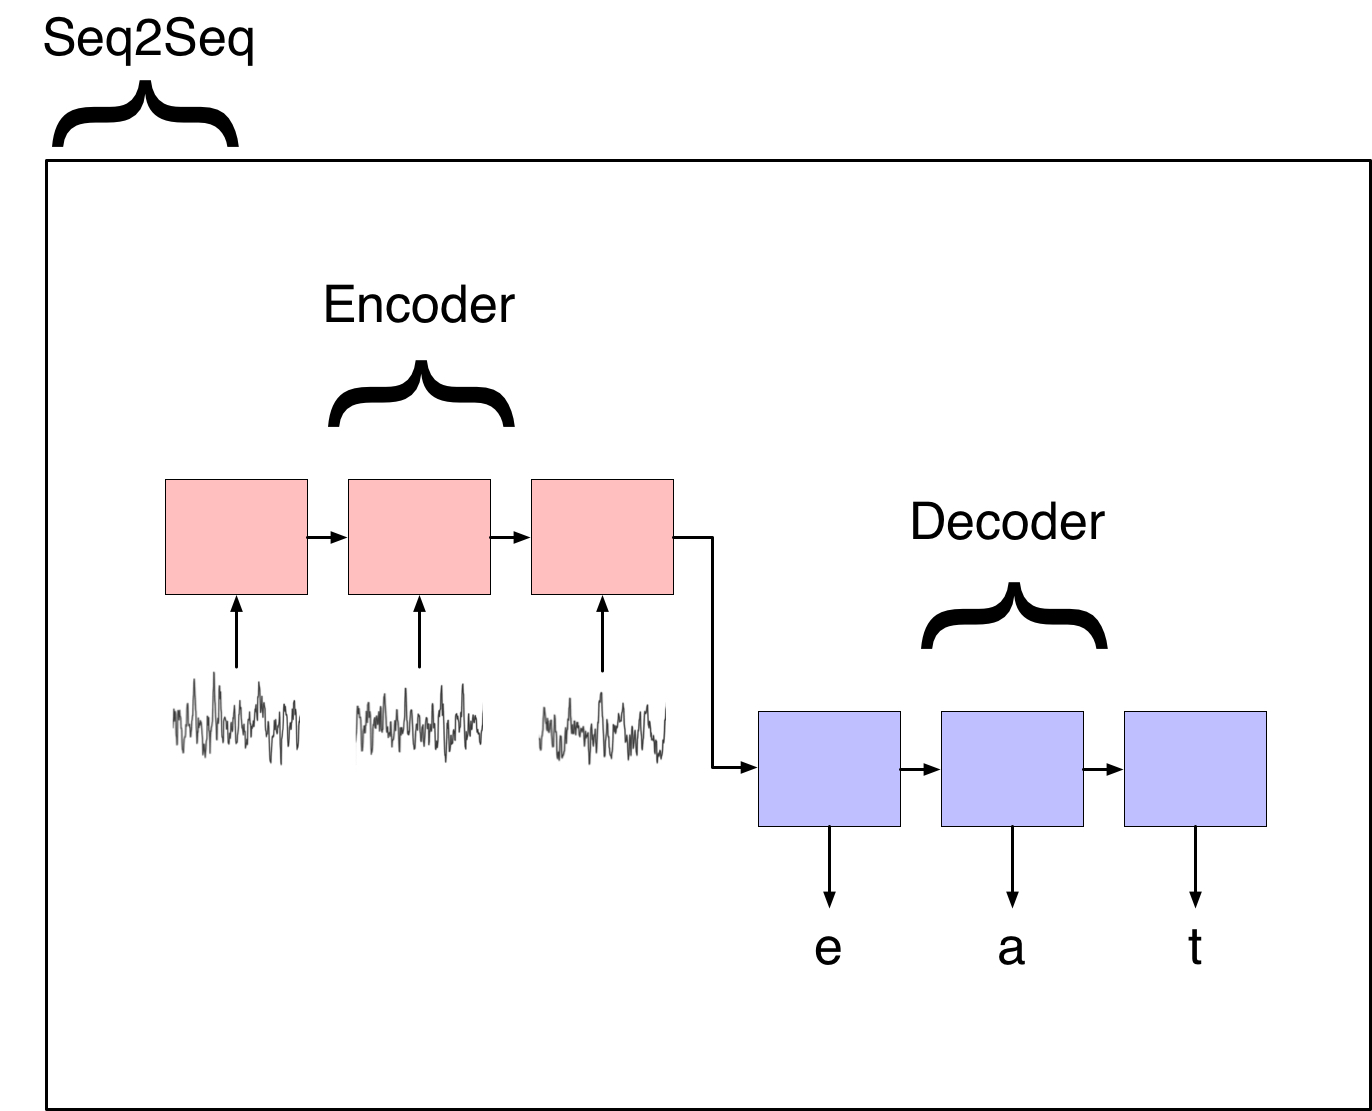
\includegraphics[width=0.75\linewidth]{fig/seq2seq_illustration.jpg}
\caption{The encoder and decoder are trained jointly in a Seq2Seq model.}
\label{learned_interp}
\end{figure}

\textbf{For this section,  you must implement a working Seq2Seq model.} Your implementation must have both the encoder and decoder as single-layer LSTMs with 50\% dropout applied to the input layer to the encoder. Every hidden dimension in your neural networks should be 128 and your embedding size should be 256. Set your optimizer to be Adam with the default PyTorch parameters. Your program should be able to run quickly and easily on a laptop due to the simplicity of our model and the limited size of our data.  


\subsection{DAgger Implementation}

As we've seen in class, DAgger is an algorithm for collecting training examples for our model by sometimes following the actions performed by an expert and sometimes following our model's decisions. 

\textbf{For this section's points, you will need to implement DAgger as described in Algorithm \ref{alg:dagger}.} Note that this algorithm allows $\beta_i$ to vary with timestep $i$. This allows us to explore various schedules for the $\beta$ parameter, including some that don't have the theoretical guarantees discussed in class. 

Please implement a general version of DAgger and then the code necessary to run DAgger with (1) a fixed $\beta$, (2) a linearly decaying $\beta$ where $\beta$ is decreased by $0.05$ after each epoch, and (3) an exponentially decaying $\beta$, where $\beta = \exp{-1 \times i}$ where $i$ is the current epoch. 

\begin{algorithm}[H]
\caption{DAgger}
\label{alg:dagger}
\begin{algorithmic}
\STATE Initialize $\mathcal{D} \gets \emptyset$.
\STATE Initialize $\hat{\pi}_1$ to any policy in $\Pi$.
\FOR{i=1 to N}
    \STATE Let $\pi_i = \beta_i \pi^* + (1-\beta_i)\hat{\pi}_i$
    \STATE Sample $T$-step trajectories using $\pi_i$.
    \STATE Get dataset $\mathcal{D}_i = \{ s, \pi^*(s)\}$ of visited states by $\pi_i$ and actions given by the expert. 
    \STATE Aggregate datasets: $\mathcal{D} \gets \mathcal{D} \cup \mathcal{D}_i$.
    \STATE Train classifier $\hat{\pi}_{i+1}$ on $\mathcal{D}$.
\ENDFOR
\RETURN best $\hat{\pi}_i$ on validation. 
\end{algorithmic}
\end{algorithm}


\subsection{Autolab Submission}
You must submit a .tar file named \lstinline{seq2seq.tar} containing \lstinline{seq2seq.py}, which contains all of your code.

You can create that file by running:
\begin{lstlisting}
tar -cvf seq2seq.tar seq2seq.py
\end{lstlisting}
from the directory containing your code.

Some additional tips: {\bf DO NOT} compress your files; you are just
creating a tarball. Do not use tar \texttt{-czvf}.  {\bf DO NOT} put
the above files in a folder and then tar the folder.  Autolab is case
sensitive, so observe that all your files should be named in {\bf
  lowercase}. You must submit this file to the corresponding homework
link on Autolab. 

Your code will \textbf{not} be autograded on Autolab. Instead, we will grade your code by hand; that is, we will read through your code in order to grade it. As such, please carefully identify major sections of the code via comments. 

\clearpage

%Collaboration Portion
\section{Collaboration Policy}

    After you have completed all other components of this assignment, report your answers to the collaboration policy questions detailed in the Academic Integrity Policies for this course.
    \begin{enumerate}
        \item Did you receive any help whatsoever from anyone in solving this assignment? If so, include full details including names of people who helped you and the exact nature of help you received.
        
        \begin{tcolorbox}[fit,height=4cm, width=15cm, blank, borderline={1pt}{-2pt},nobeforeafter]
        % Place your solution between the comment lines below.
        % Do not modify the tcolorbox.
        % ----------------------------------------------------
        % STUDENT SOLUTION HERE
        % ----------------------------------------------------
       \end{tcolorbox}
        \item Did you give any help whatsoever to anyone in solving this assignment? If so, include full details including names of people you helped and the exact nature of help you offered.
        
        \begin{tcolorbox}[fit,height=4cm, width=15cm, blank, borderline={1pt}{-2pt},nobeforeafter]
        % Place your solution between the comment lines below.
        % Do not modify the tcolorbox.
        % ----------------------------------------------------
        % STUDENT SOLUTION HERE
        % ----------------------------------------------------
       \end{tcolorbox}
        \item Did you find or come across code that implements any part of this assignment? If so, include full details including the source of the code and how you used it in the assignment.
        
        \begin{tcolorbox}[fit,height=4cm, width=15cm, blank, borderline={1pt}{-2pt},nobeforeafter]
        % Place your solution between the comment lines below.
        % Do not modify the tcolorbox.
        % ----------------------------------------------------
        % STUDENT SOLUTION HERE
        % ----------------------------------------------------
       \end{tcolorbox}
    \end{enumerate}

\end{document}